% Chapter 2: Background

% Length: aim for 10-15 pages

This chapter presents the different background topics of the thesis work, which are the long-tailed datasets, model architectures \textit{Convolutional Neural Networks (CNN)} and \textit{Visual Transformers (VT)}, the deep long-tailed learning methods \textit{Class Re-balancing (CR)}, \textit{Information Augmentation (IA)}, 
and \textit{Module Improvement (MI)}. These topics will be explained for the reader.\\

Mention image classification, as it is the primary goal of this thesis. 

\section{Long-Tailed Datasets}
Long-tailed datasets pose significant challenges in deep learning, as they represent an extreme form of class imbalance. Addressing these challenges is central to this thesis, which explores methods to improve model performance on underrepresented classes. This section outlines the structure of long-tailed distributions and their implications.

A balanced dataset is one where all classes are evenly represented, whereas imbalanced datasets feature varying sample sizes across classes. Long-tailed datasets are characterized by a significant class imbalance, where a few dominant classes account for most samples (head classes), while the majority of classes are underrepresented (tail classes) as depicted in Figure \ref{fig:lt_distribution}. This  distribution is common for real-world datasets \cite{Newman_2005, liu2019largescalelongtailedrecognitionopen}. For example, the iNaturalist, a popular benchmark for image classification, exhibits a long-tailed distribution of species \cite{vanhorn2018inaturalistspeciesclassificationdetection}. Other benchmarks are constructed by sampling from datasets such as ImageNet \cite{ImageNet2009} and CIFAR-100 \cite{krizhevsky2009learning} using a Pareto distribution, which simulates long-tailed class distributions with a power-law decay \cite{zhang2023deep, dealvis2024surveydeeplongtailclassification,cao2019learningimbalanceddatasetslabeldistributionaware}.

One such benchmark, CIFAR100-LT \cite{cao2019learningimbalanceddatasetslabeldistributionaware}, derived from the CIFAR-100 dataset \cite{krizhevsky2009learning}, serves as the primary dataset for the experiments conducted in this thesis. CIFAR-100 is a widely used benchmark in classification research due to its diverse class representation and manageable size. It consists of 60,000 32x32 color images divided into 100 classes, each with 600 samples. These are further split into 500 training images and 100 testing images per class. CIFAR100-LT is created by reducing the number of samples in certain classes of CIFAR-100 following a Pareto distribution, introducing significant class imbalance. This makes it an ideal benchmark for studying the challenges posed by long-tailed datasets.  

\begin{figure}[ht]
    \centering
    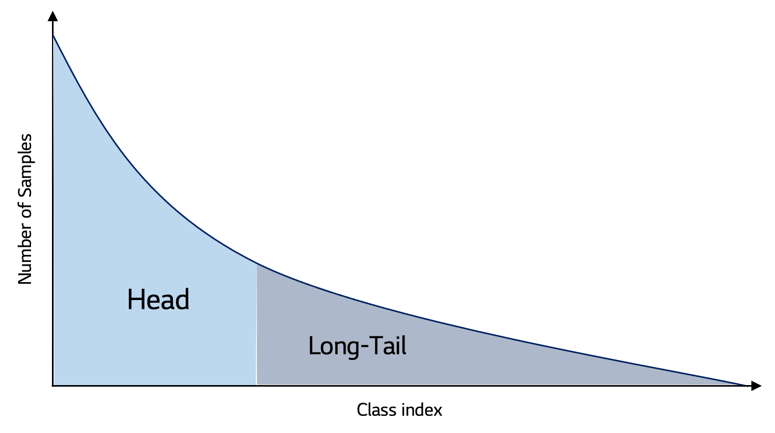
\includegraphics[width=0.8\textwidth]{Images/long_tail_distribution.png} 
    \caption{Illustration of a long-tailed distribution. Figure from \cite{lgresearch257}.}
    \label{fig:lt_distribution} % Use a unique label for referencing the figure
\end{figure}

Class imbalance has a profound impact on model performance compared to evenly distributed datasets \cite{vanhorn2017deviltailsfinegrainedclassification, cui2019classbalancedlossbasedeffective}. Deep networks trained on long-tailed datasets often exhibit biased performance, favoring head classes while performing poorly on tail classes \cite{zhang2023deep}. Zhang et al. (2023) provide a comprehensive survey of methods addressing this challenge, categorizing current approaches into three main groups: class re-balancing, information augmentation, and module improvement. These methods will be further explored in section \ref{sec:lt_methods}. 


%===================================================================================

\section{Model Architechtures}
Deep learning has revolutionized image classification by introducing models capable of learning complex patterns and representations from data. Among these, Convolutional Neural Networks (CNNs) and Visual Transformers (VTs) stand out as the primary architectures used in this thesis. This section provides a theoretical foundation for these models, focusing on the specific architectures utilized: MobileNetV2 \cite{sandler2018mobilenetv2}, ResNet50V2 \cite{he2016}, and ConvNeXt Base \cite{todi2023convnext} as the CNN architectures, and ViT-B/16 \cite{dosovitskiy2021imageworth16x16words} as the VT architecture.

\subsection{Introdution to Neural Networks}
Before the introduction of Convolutional Neural Networks (CNNs) and, more recently, Vision Transformers (ViTs), the standard approach for image classification involved flattening a two-dimensional image matrix into a one-dimensional array and passing it through a Multilayer Perceptron (MLP), also known as a feed-forward neural network. MLPs are fully connected neural networks composed of an input layer, output layer, and one or more hidden layers. Being fully connected means that each neuron in a given layer is connected to all neurons in the next layer, forming a dense network. These connections are associated with weights and biases, which the network learns during training. Input features are fed into the input layer, propagated through hidden layers that add complexity to model nonlinear relationships, and yield predictions in the output layer. Known as universal approximators, MLPs can approximate any continuous function given sufficient neurons in the hidden layers \cite{zhang2023dive}.

To illustrate the structure of a neural network, figure \ref{fig:cnn_layers} shows an example of a feed-forward neural network with three input neurons, two hidden layers, each with four neurons, and two output neurons. This architecture could be used, for instance, to classify images of cats and dogs based on three input features, such as height, weight, and width of the animals. The input propagates through the network, with each neuron computing a weighted sum of its inputs followed by an optional nonlinearity. The final output is a prediction, where the class corresponding to the neuron with the highest value is chosen.

\begin{figure}[ht]
    \centering
    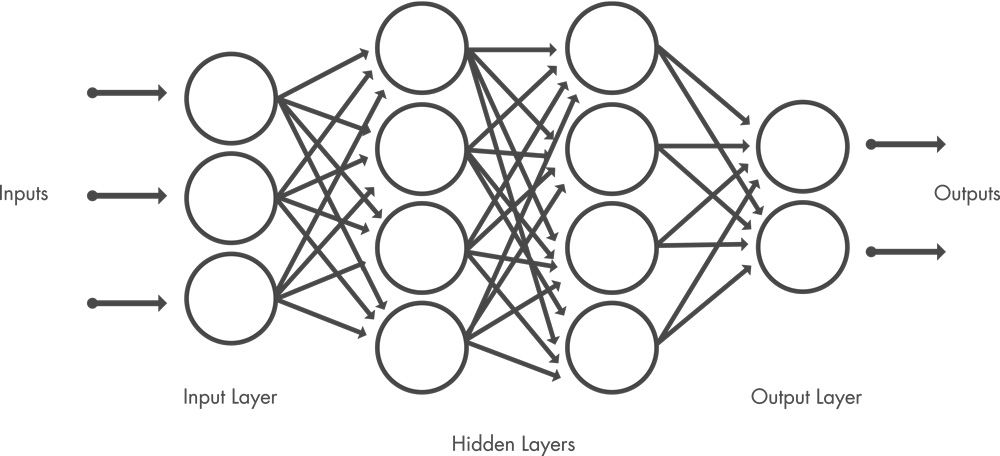
\includegraphics[width=0.8\textwidth]{Images/cnn_layers.jpg} 
    \caption{Layers of a convolutional neural network. Figure from \cite{mathworks_cnn}.}
    \label{fig:cnn_layers}
\end{figure}

However, this simple neural network becomes insufficient for more complex problems, such as image classification, as it requires an increasing number of parameters. This limitation was addressed by CNNs, which introduced convolutional and pooling layers to effectively preserve and utilize the spatial information of pixels in two-dimensional images \cite{zhang2023dive}.

\subsection{Convolutional Neural Networks}

% What are CNNs?
% Historical context.
% Input data.
% Output data.
% Layers.

% Before the CNNS, the standard was to flatten the image from two dimensional matrix into a one dimensional array and pass it through a feed-forward neural network in order to classify the image. As the image is converted into one dimension, naturally, spacial information in the image is lost. 

% As is common for all neural networks, they are made up of neurons with learnable weights and biases, and has an input layer and an output layer with several hidden layers in between, where each hidden layer can have an arbitrary amount of neurons. Each neron recieves some inputs, perfom dot product and optionally follows it with nonlinearity.

%  A simple neural network is illustrated in figure \ref{fig:cnn_layers}, which shows an NN with three input neurons, two hidden layers with four neurons each, and an output layer of two neurons. The example in figure \ref{fig:cnn_layers} could be a neural network designed to classify cats and dogs based on three parameters. The parameters could be height, weight, and nose length of the pet. This data would propagate through the NN and the result would be the value of the two output neurons. The output with the highest value would be intrepreted as the class of the given input data, either a cat or a dog. The idea is that a neural network functions as a universal approximator, and without the hidden layers, it is just a linear function \cite{zhang2023dive}. The hidden layers introduce nonlinearity  
 


 A convolutional neural network is a neural network architecture for deep learning that gained popularity after being introduced by LeCun et al. in 1995 \cite{lecun1995}. It is designed to recognize patterns in images for classification, as CNNs preserve the two dimensional input of an image, preserving the idea that nearby pixels are related. 




\begin{figure}[ht]
    \centering
    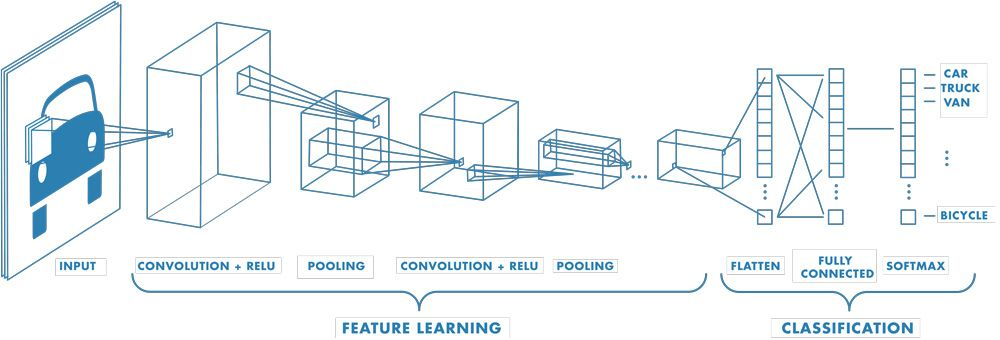
\includegraphics[width=0.8\textwidth]{Images/CNN_illustration.jpg} 
    \caption{Illustration of a convolutional neural network. Figure from \cite{mathworks_cnn}.}
    \label{fig:cnn_illustration}
\end{figure}

\subsubsection{MobileNetV2 Architechture}

MobileNetV2 is a lightweight CNN architecture designed for efficient mobile and edge computing applications \cite{sandler2018mobilenetv2}. It introduces two key innovations:

Inverted Residuals: Use of shortcut connections between thin bottleneck layers to improve performance while maintaining low computational cost.
Linear Bottlenecks: Avoiding non-linearities in narrow layers to preserve information. MobileNetV2 is particularly suited for image classification tasks on resource-constrained devices and is used in this thesis for its efficiency and effectiveness in feature extraction.

\subsubsection{ResNet50V2 Architechture}
ResNet50V2 is a variant of the ResNet (Residual Network) architecture, which introduced the concept of residual learning to address the vanishing gradient problem in deep networks \cite{he2016}. Key features include:

Residual Connections: Allow gradients to flow more effectively through deeper layers.
Improved Training Dynamics: Incorporates pre-activation, leading to smoother optimization. ResNet50V2’s ability to extract hierarchical features and its robustness to overfitting make it a popular choice for image classification tasks.

\subsubsection{ConvNeXt Base Architechture}
ConvNeXt Base is a modernized CNN architecture inspired by insights from transformer-based models, designed to achieve competitive performance while retaining the efficiency of CNNs \cite{todi2023convnext}. Notable features include:

Simplified Design: Incorporates architectural refinements such as depthwise convolutions and LayerNorm.
Enhanced Efficiency: Balances accuracy and computational cost, bridging the gap between traditional CNNs and transformer-based models. ConvNeXt Base represents a state-of-the-art approach to CNN design, making it a compelling choice for this thesis.


\subsection{Visual Transformers}
Explain their advantages over CNNs for certain tasks.
Mention why they are relevant for handling long-tailed datasets.

\subsubsection{ViT-B/16 Architecture}
ViT-B/16 is a Visual Transformer model that leverages the transformer architecture for image classification \cite{dosovitskiy2021imageworth16x16words}. Key characteristics include:

Patch Embeddings: Images are divided into 16x16 patches, which are then flattened and embedded.
Self-Attention Mechanism: Captures global dependencies and relationships between image regions.
Scalability: Performs particularly well on large-scale datasets, where its global attention mechanism can fully exploit the available data. ViT-B/16 exemplifies the application of transformers in computer vision and is used in this thesis to explore the capabilities of attention-based architectures.

%====================================================================================

\section{Classic Long-Tailed Methods}
\label{sec:lt_methods}
Introduce the three methods (CR, IA, MI) with a brief explanation of their purpose.\\

Following the paper \textit{Deep Long-Tailed Learning: A Survey} \cite{zhang2023deep}, the existing deep long-tailed learning methods are grouped into three main categories based on their technical approach: class re-balancing, information augmentation, and module improvement. These categories are further divided onto sub-categories: re-sampling, class-sensitive learning, logit adjustment, transfer learning, data augmentation, representation learning, classifier desing, decoupled training, and ensemble learning as shown on figure \ref{fig:lt_main_categories}. This thesis does not aim to examine all the beforementioned method, but aims to find a deep learning approach to a specific problem. The backgrounds of the methods used in this thesis are described in this section.

\begin{figure}[ht]
    \centering
    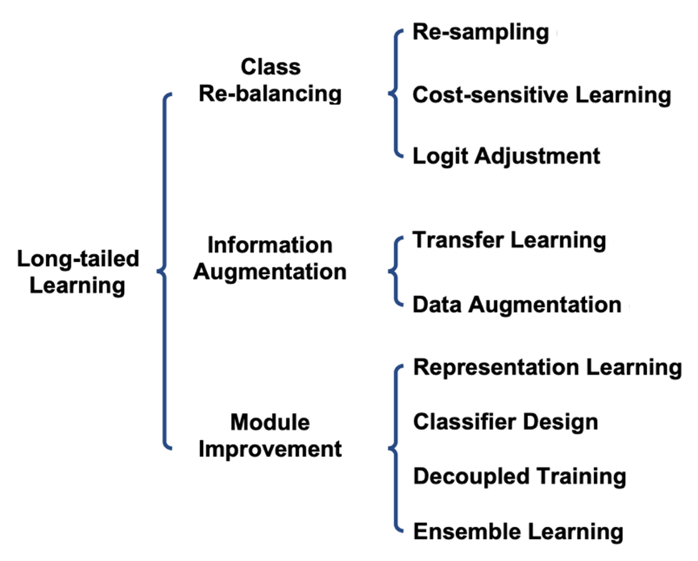
\includegraphics[width=0.8\textwidth]{Images/lt_methods_categories.png} 
    \caption{Long-tailed categories as described by \textit{Zhang et al.} \cite{zhang2023deep}.}
    \label{fig:lt_main_categories} % Use a unique label for referencing the figure
\end{figure}

\subsection{Class Re-balancing}
The class re-balancing method aims to re-balance the effect of the imbalanced training dataset, and has three main sub-categories: re-sampling, class-sensitive learning, and logit adjustment \cite{zhang2023deep}. 

\subsubsection{Re-sampling}
The traditional way to sample when training deep networks is bases on mini-batch gradient descent with random sampling. This means that each sample has an equal probability of being sampled. When sampling from an imbalanced dataset, samples from head classes naturally occur more often, and thus have higher chance of being sampled than samples from tail classes, making the resulting deep models biased towards head classes. Re-sampling is a method that adresses this problem by adjusting the number of samples per class in each sample batch for model training. 

\subsubsection{Class-sensitive Learning}
Class-sensitive learning incorporates strategies to adjust the loss function, making it more sensitive to the imbalanced nature of the dataset. This approach directly modifies the optimization process to prioritize learning from under-represented tail classes.

TODO: Mention re-weighting and re-margining.
Table/overview of loss functions as in the paper.


\subsubsection{Loss Functions for Class-Sensitive Learning}
The loss function serves as a measure of the model's fitness to the data, quantifying the distance between the actual and predicted values of the target. Typically, the loss is represented as a nonnegative value, where smaller values indicate a better fit, and a perfect fit corresponds to a loss of zero \cite{zhang2023dive}.

Conventional training of deep networks using the softmax cross-entropy loss often overlooks class imbalance. This results in uneven gradients for different classes, leading to suboptimal performance on underrepresented classes. To mitigate this issue, modifications to the loss function are introduced to ensure a more balanced contribution from each class during training. One such technique is re-weighting which adjusts the training loss for different classes by assigning a specific weight to each class \cite{zhang2023deep}. The softmax cross-entropy loss is used as a baseline, and is described below along with the loss functions for re-weighting.

\myindent \textbf{Softmax Cross-Entropy Loss}
The \textit{Softmax-Cross-Entropy loss}, often referred to as \textit{softmax loss}, is a widely used combination for training deep neural networks in classification tasks, including image classification. It is particularly effective for multi-class problems, where the goal is to assign an input image to one of several predefined categories \cite{cs231n} \cite{pytorch_crossentropy}.

The \textit{Softmax} function transforms the raw output scores (logits) of the final layer of a neural network into a probability distribution over \( K \) classes. For an input \( \mathbf{z} = [z_1, z_2, \dots, z_K] \), the Softmax function for class \( i \) is defined as:

\begin{equation}
    P(y = i \mid \mathbf{z}) = \frac{\exp(z_i)}{\sum_{j=1}^{K} \exp(z_j)}
\end{equation}

Here, \( \exp(z_i) \) ensures that all values are positive, and dividing by the sum normalizes the probabilities so that they sum to 1. This normalization is crucial for classification, as it allows the network's outputs to represent the likelihood of each class.

The \textit{Cross-Entropy loss} measures the difference between the predicted probability distribution \( \mathbf{P} \) (produced by Softmax) and the true distribution \( \mathbf{y} \) (the one-hot encoded ground truth). It is defined as:

\begin{equation}
    \mathcal{L}_{\text{CE}} = -\sum_{i=1}^{K} y_i \log(P(y = i \mid \mathbf{z}))
\end{equation}


For a single example where the true class is \( c \), this simplifies to:

\begin{equation}
    \mathcal{L}_{\text{CE}} = -\log(P(y = c \mid \mathbf{z}))
\end{equation}


This formulation penalizes incorrect predictions by heavily weighting the log of the predicted probability for the true class. The loss is minimized when the predicted probability \( P(y = c \mid \mathbf{z}) \) approaches 1, indicating high confidence in the correct class.

This combination has become the de facto standard for image classification tasks, providing a robust and mathematically sound framework for training deep neural networks.


\myindent \textbf{Weighted Softmax Cross-Entropy Loss}
The \textit{Weighted Softmax Cross-Entropy loss}, often referred to as \textit{weighted softmax loss}, is a variant of the standard softmax cross-entropy loss, designed to address imbalanced datasets \cite{pytorch_crossentropy} \cite{lin2018focallossdenseobject}. By assigning different weights to each class, this method ensures that underrepresented classes contribute more to the overall loss, improving the model's performance on minority classes. The weighted cross-entropy loss applies class-specific weights to the standard cross-entropy formulation. It is defined as:

\begin{equation}
    \mathcal{L}_{\text{WCE}} = -\sum_{i=1}^{K} w_i y_i \log(P(y = i \mid \mathbf{z}))
\end{equation}

Where \( w_i \) is the weight for class \( i \), reflecting its relative importance, \( y_i \) is the one-hot encoded true label for class \( i \), and \( P(y = i \mid \mathbf{z}) \) is the predicted probability for class \( i \).

For a single example where the true class is \( c \), the loss simplifies to:

\begin{equation}
    \mathcal{L}_{\text{WCE}} = -w_c \log(P(y = c \mid \mathbf{z}))
\end{equation}

This weighted formulation ensures that minority classes contribute more to the overall loss, addressing the imbalance during training and improving the model's performance on underrepresented classes.

\myindent \textbf{Focal Loss}
Focal Loss, introduced by Lin et al. (2017) \cite{lin2018focallossdenseobject}, addresses the challenges of extreme class imbalance in classification tasks by dynamically scaling the standard cross-entropy loss. Focal Loss mitigates the issue of imbalanced datasets by down-weighting the loss contributions from well-classified examples and focusing on misclassified examples during training.

% For multiclass classification, the focal loss is formulated as:

% \begin{equation}
%     \mathcal{L}_{\text{FL}} = - \frac{1}{N} \sum_{i=1}^{N} \sum_{c=1}^{K} \alpha_c (1 - p_{i,c})^\gamma \log(p_{i,c}),
% \end{equation}

% where \( N \) is the number of samples, \( K \) is the total number of classes, \( p_{i,c} \) is the predicted probability for class \( c \) for the \( i \)-th sample, typically obtained via a softmax function, \( \alpha_c \) is a weighting factor for class \( c \), \( \gamma \geq 0 \) is the focusing parameter, which adjusts the scaling effect of \( (1 - p_{i,c})^\gamma \). A higher \( \gamma \) increases the model's focus on harder examples, and \( \log(p_{i,c}) \) is the standard cross-entropy loss for the true class.


% The term \( (1 - p_{i,c})^\gamma \) serves as a modulating factor that reduces the contribution of well-classified examples, where \( p_{i,c} \) is high, to the total loss. This enables the model to focus more on examples with lower predicted probabilities, which are typically harder to classify. The parameter \( \alpha_c \) further adjusts the loss to account for class imbalance, ensuring that minority classes receive adequate attention during training.


\myindent \textbf{Class-Balanced Loss} \textit{Class-balanced loss}, introduced by Cui et al. (2019) \cite{cui2019classbalancedlossbasedeffective}, ...

\myindent \textbf{Balanced Softmax Loss} \textit{Balanced Softmax loss}, introduced by Ren et al. (2020) \cite{ren2020balancedmetasoftmaxlongtailedvisual}, ...

\myindent \textbf{LDAM Loss} \textit{LDAM loss}, introduced by Cao et al. (2019) \cite{cao2019learningimbalanceddatasetslabeldistributionaware}, ...

\myindent \textbf{Equalization Loss} \textit{Equalization loss}, introduced by Tan et al. (2020) \cite{tan2020equalizationlosslongtailedobject}, ...


\subsection{Information Augmentation}
Data augmentation techniques tailored for long-tailed datasets.

\subsubsection{Transfer Learning}

\subsubsection{Data Augmentation}



\subsection{Module Improvement}
Architectural changes to improve tail-class representation.